% This is samplepaper.tex, a sample chapter demonstrating the
% LLNCS macro package for Springer Computer Science proceedings;
% Version 2.20 of 2017/10/04
%
\documentclass[runningheads]{llncs}
%
\usepackage{hyperref}   % hyperlinks
\usepackage{graphicx}
\usepackage{algorithm}
\usepackage[noend]{algpseudocode}
\usepackage{multirow}
\usepackage{longtable}

% Used for displaying a sample figure. If possible, figure files should
% be included in EPS format.
%
% If you use the hyperref package, please uncomment the following line
% to display URLs in blue roman font according to Springer's eBook style:
% \renewcommand\UrlFont{\color{blue}\rmfamily}

% ------------------------------------------------------------------------------

\begin{document}
%
\title{Colorarea grafurilor}
%
\author{Cărămidă Iustina-Andreea - 322CA}
%
\institute{Facultatea de Automatică și Calculatoare \\
Universitatea Politehnica București \\
\email{iustina.caramida@stud.acs.upb.ro}
}
%
\maketitle              % typeset the header of the contribution
%
\begin{abstract}
    Problema colorării nodurilor unui graf (\textit{graph coloring - GCP} sau \textit{colorarea grafurilor})
    este una dintre cele mai importante probleme, fapt datorat numărului mare de situații din viața reală
    care se pot rezuma la o problemă de colorare a unui graf. În această temă, voi prezenta câteva comparări 
    între diferiți algoritmi dedicați acestei probleme, precum Greedy, Dsatur și RLF din 
    punct de vedere al timpului de execuție, al memoriei folosite și al performanței în raport cu numărul 
    de noduri și muchii.


\keywords{Brute-Force \and Greedy \and DSatur \and RLF \and Colorarea grafurilor.}
\end{abstract}

% ------------------------------------------------------------------------------

\section{Introducere}
\subsection{Descrierea problemei}

\quad Colorarea grafurilor este o problemă centrală în teoria grafurilor \cite{1}. Ea 
constă în alegerea unui set de culori pentru nodurile unui graf, astfel încât 
niciun nod adiacent să nu primească aceeași culoare.

Problema colorării graficului a început cu încercarea lui 
Francis Guthries de a colora toate țările pe harta Angliei. 
Acesta a presupus inițial că patru culori sunt suficiente pentru a procesa orice 
hartă, astfel încât să nu fie asociate două țări vecine
cu aceeasi culoare. Această sarcină este doar una dintre cele peste 200 de probleme
\cite{2}, legate de aria analizei grafice cromatice,
iar această situație poate fi tradusă prin colorarea fiecărui vârf
dintr-un graf în care marginile sale ar reprezenta vecinătatea
dintre două regiuni \cite{3}.

Colorarea grafurilor este o problemă de tip NP-hard bine studiată cu aplicații 
importante în optimizarea combinatorie și într-un domeniu de cercetare activ, cu 
multe aplicații practice \cite{4} în inginerie, cum ar fi \textit{alocarea registrelor}, 
\textit{atribuirea frecvenței}, \textit{potrivirea șablonului} și \textit{programări}. 
În consecință, colorarea grafurilor a fost subiectul unor cercetări intense \cite{5} \cite{2}.

Un exemplu de o problemă de colorare a grafurilor este planificarea examenelor, unde
fiecare examen este reprezentat de un nod și fiecare legătură dintre nodiri reprezintă
o interzicere de a planifica examenele. Astfel, colorarea grafului reprezintă planificarea
examenelelor, astfel încât două examene care nu pot fi planificate în același timp să fie
colorate diferit. În acest caz, numărul minim de culori necesare pentru a colora graful
este egal cu numărul minim de zile necesare pentru a planifica examenele. \cite{6}

Colorarea grafurilor este asociată cu două tipuri de colorare: colorarea vârfurilor 
și colorarea marginilor. Scopul ambelor tipuri de colorare este de a colora întregul graf fără
conflicte. Prin urmare, vârfurile adiacente sau muchiile adiacente trebuie
să fie în culori diferite. Numărul cel mai mic de culori necesare 
pentru a colora graful se numește \textbf{număr cromatic}.
Pe măsură ce numărul de vârfuri sau muchii dintr-un graf crește,
complexitatea problemei crește și ea. Din această cauză, fiecare
algoritmul nu poate găsi numărul cromatic exact  
și pot fi, de asemenea, diferențe în timpul lor de execuție \cite{7}. Pentru a obține 
o soluție mai bună pentru colorarea grafurilor, mulți algoritmi euristici și meta
euristici au fost inventați \cite{8}.
% 
\subsection{Specificarea algoritmilor aleși}

\textbf{\textit{Cerință:}} Fie un graf neorientat G cu N noduri și M muchii. Problema cere să asociem o culoare 
fiecărui nod, astfel încât oricare două noduri adiacente (conectate printr-o muchie directă) 
să aibă culori diferite. Care este numărul minim de culori necesare pentru a colora 
toate nodurile conform restricției menționate anterior? \cite{9}

\subsubsection{Brute Force:}
Când încercăm să oferim o soluție la această problemă, primul instinct este de a
folosi o abordare ”Brute Force”. Acest lucru ar duce la o soluție, care ar fi 
din punct de vedere al timpului de execuție exponențială, făcând această soluție 
inutilă pentru cazuri mari. A spune că nu putem găsi un algoritm eficient 
deoarece acesta nu există ar fi la fel ca și când am spune că problema nu are 
nicio soluție eficientă \cite{10}.
În prezent, există algoritmi care se ocupă să rezolve problema colorării grafurilor, 
deși obțin un număr cromatic apropiat de ale grafului în schimbul unui timp
rezonabil sau rezultate rapide care sunt suficient de utile \cite{11}.

\subsubsection{Greedy Algorithm:}
Logica algoritmului ia vârfurile grafului unul câte unul, urmând o ordine 
(care poate fi aleatorie) și atribuie prima culoare disponibilă fiecărui vârf \cite{12}. 
Deoarece este un algoritm euristic, soluția oferită de acesta poate să nu fie optimă.
Cu toate acestea, o alegere corectă a ordinii vârfurilor pentru
colorarea lor poate oferi o soluție optimă pentru orice graf. În
practică, algoritmul Greedy produce soluții rapid practicabile, deși aceste soluții 
pot fi “sărace” pe baza numărului de culori pe care algoritmul le cere, în comparație cu
numărul cromatic al grafului.

\subsubsection{DSatur Algorithm:}
Algoritmul DSatur (abreviere din engleză pentru “Degree Saturation”), 
propus de Brelaz (1979), se comportă foarte asemănător cu
algoritmul Greedy, cu excepția că, în acest caz,
ordonarea vârfurilor este generată de algoritmul însuși.
La fel ca în algoritmul Greedy, ordonarea a fost decisă
înainte ca orice vârf să fie colorat, ordinea vârfurilor fiind decisă euristic pe baza
caracteristicilor colorării parțiale a grafului la
momentul în care se selectează fiecare dintre vârfuri \cite{13}. 
În cel mai rău caz, complexitatea sa are aceeași situație ca și în
Algoritmul Greedy, deși în practică poate fi luat în considerare
și faptul că monitorizare saturaţiei vârfurilor necolorate
produce o complexitate puțin mai mare. Este de reținut că
Algoritmul DSatur este \textbf{exact} pentru grafurile bipartite \cite{14}.

\subsubsection{RLF Algorithm:}
Algoritmul RLF (abreviere din engleză pentru “Recursive Largest First”), propus
de Leighton (1979), lucrează prin colorarea unui graf cu o singură culoare
pentru fiecare iterație a algoritmului, în loc de un vârf per
repetare. În fiecare iterație, algoritmul caută seturi de
vârfuri independente din graf, care vor fi asociate
cu aceeași culoare. Acel set independent a fost eliminat
din graf, iar subgraful rămas va continua
în același mod, până când subgraful menționat este gol, caz în care
toate vârfurile vor fi atribuite unei culori, producând astfel o
soluție ce satisface toate cerințele \cite{12}.

\subsection{Evaluarea soluțiilor}
Sursele vor fi testate pe grafuri de dimensiuni diferite, de la 10 la 2 000 de noduri,
cu un număr de muchii de la 10 la 1 000 000. Pentru fiecare graf se va genera o
configurație aleatoare de noduri și muchii, iar apoi se va testa performanța
algoritmilor pe aceste grafuri. Pentru fiecare algoritm, se va calcula timpul de
execuție și numărul de culori folosite pentru a colora graful.

\section{Prezentarea soluțiilor}
\subsection{Algoritmul Brute Force}
Algoritmul Brute Force este un algoritm care se bazează pe forță bruta, adică
parcurge toate posibilitățile de colorare a grafului și alege cea mai bună
soluție. Complexitatea acestui algoritm este de $O(n^m)$, unde $n$ este numărul de noduri și $m$ este
numărul de culori. Pentru grafuri cu un număr mare de noduri, complexitatea
acestui algoritm este foarte mare, de aceea nu este folosit în practică. Pe de altă parte,
algoritmul este exact, adică oferă întotdeauna o soluție optimă. Un pseudocod al
algoritmului este prezentat în Pseudocodul~\ref{alg1}.

\begin{algorithm}
\caption{Brute Force Algorithm}
\label{alg1}
\begin{algorithmic}[1]
\Procedure{BruteForce}{$G$} \Return $List\langle int\rangle $ 
\State $List\langle int\rangle $ $colors = new List\langle int\rangle $ \Comment{List of colors}
\State $int$ $maxColors = 0$ \Comment{Number of colors}
\State $int$ $maxColorsIndex = 0$ \Comment{Index of the best solution}
\algstore{bkbreak}
\end{algorithmic}
\end{algorithm}

\addtocounter{algorithm}{-1}
\begin{algorithm}
\caption{Brute Force Algorithm}
\begin{algorithmic}[1]
\algrestore{bkbreak}
\State $int$ $i = 0$ \Comment{Index of the current solution}
\State $int$ $n = G.GetNumberOfNodes()$ \Comment{Number of nodes}
\State $int$ $m = G.GetNumberOfColors()$ \Comment{Number of colors}
\State $int$ $max = pow(m, n)$ \Comment{Number of possible solutions}
\While{$i < max$}
\State $colors = G.GetColors()$
\State $int$ $currentColors = colors.Count()$
\If{$currentColors > maxColors$}
\State $maxColors = currentColors$
\State $maxColorsIndex = i$
\EndIf
\State $i++$
\EndWhile
\State $colors = G.GetColors(maxColorsIndex)$
\State \Return $colors$
\EndProcedure
\end{algorithmic}
\end{algorithm}


\subsection{Algoritmul Greedy}
Algoritmul Greedy este un algoritm care alege mereu cea mai bună soluție la
momentul curent, fără a ține cont de soluțiile viitoare.
Un pseudocod al algoritmului este prezentat în
Pseudocodul~\ref{alg2}.


\begin{algorithm} 
\caption{Greedy Algorithm}
\label{alg2}
\begin{algorithmic}[1]
\Procedure{Greedy}{$G$}
\Require{$S$ = Class Set, $V$ = Colorless vertices in random order}
\Ensure{$S$ = $\emptyset$}
\For{$v \in V$}
\For{$i$ to $S.lenght$}
\If {$NonConflitiveEdges(v \cup S_i)$}
\State $AssignClass(v, S_i)$
\State $Next Vertex$
\EndIf
\EndFor
\If {$NotColored(v)$}
\State $S_{i+1} = NewClass$
\State $AssignClass(v, S_{i+1})$
\State {Next Vertex}
\EndIf
\EndFor
\EndProcedure
\end{algorithmic}
\end{algorithm}

În algoritmul Greedy, așa cum se poate vedea în pseudocod,
se folosește o permutare inițială care este generată aleatoriu și în
care este colorat fiecare vârf, comparând în fiecare caz dacă acesta
poate fi inclus într-o culoare fără a provoca conflicte. Pentru a analiza
algoritmul în cel mai rău caz, vom presupune că fiecare vârf este 
verificat cu fiecare culoare înainte de a fi colorat,
ce ne dă un polinom care este
\begin{equation} P(x) = n(n+1)/2. \end{equation} Polinomul
se obţine din faptul că fiecare vârf, înainte de a fi colorat,
trebuie să se compare cu toate culorile actuale:
\begin{equation} P = 0 + 1 + 2 + . . . + n = n(n + 1)/2 \end{equation}

În cele din urmă, vom avea o complexitate de $O(n^2)$, unde $n$ este numărul
de noduri. Este necesar să afirmăm că algoritmul Greedy, deși calculează
numărul cromatic aproximativ, acest lucru va depinde direct de permutarea
inițială pe care o avem. Cu algoritmul următor vom vedea tehnici care ne
permit să îmbunătățim modul de a alege vârfurile pentru a obține soluții
mai bune și mai apropiate de numărul cromatic.

\subsection{Algoritmul DSatur}
Algoritmul DSatur este un algoritm care alege mereu nodul cu cea mai mare
valoare de saturație, adică nodul care are cel mai mare număr de vecini cu
aceeași culoare. Un pseudocod al algoritmului este prezentat în Pseudocodul~\ref{alg3}.
\begin{algorithm}
\caption{DSatur Algorithm}
\label{alg3}
\begin{algorithmic}[1]
\Procedure{DSatur}{$G$}
\Require{$S$ = Class Set, $V$ = Non-colored vertices}
\Ensure{$S$ = $\emptyset$}
\While {$V \neq \emptyset$}
\State $v = MaxSaturation(V)$
\For {$i$ to $S.lenght$}
\If {$NonConflitiveEdges(v \cup S_i)$}
\State $AssignClass(v, S_i)$
\State {Next Vertex (break)}
\EndIf
\If {$NotColored(v)$}
\State $S_{i+1} = NewClass$
\State $AssignClass(v, S_{i+1})$
\State $Remove(v, V)$
\State {Next Vertex}
\EndIf
\EndFor
\EndWhile
\EndProcedure
\end{algorithmic}
\end{algorithm}

Se poate observa din pseudocod că acest algoritm este foarte asemănător cu algoritmul
Greedy, însă puterea algoritmului DSatur constă în prioritatea dată nodurilor cu cea mai
mare saturație. Astfel, aceste noduri mai restrânse sunt colorate înainte de restul nodurilor,
care nu au aceste “restricții”. Complexitatea algoritmului este similară cu cea a algoritmului
Greedy, deoarece este foarte asemănător în cod, însă are și calcule suplimentare pentru a
obține saturația nodurilor, însă acestea nu afectează direct complexitatea totală a algoritmului,
care este totuși $O(n^2)$. 

Trebuie punctat faptul că, deși algoritmul DSatur are o performanță mai bună,
acesta are și cazuri în care obține o soluție
mai proastă decât algoritmul Greedy. Aceasta se poate observa în \cite{15} unde se arată că o
distribuția neadecvată a vârfurilor este dificil de colorat cu algoritmul DSatur.

\subsection{Algoritmul RLF}
Algoritmul RLF caută să coloreze toate vârfurile disponibile în momentul în care
acestea nu afectează niciun conflict al aceleiași culori. De asemenea, acordă
prioritate vârfurilor care au un grad mai mare, acordând astfel prioritate tipului
nostru de restricție prevăzut pentru această euristică. Algoritmul RLF are
o complexitate în cel mai rău caz mai mare decât cea a algorimului Greedy sau
DSatur, aceasta fiind o complexitate dovedită și de Leighton (1979) - $O(n^3)$.
Cu toate acestea acest algoritm are și o îmbunătățire a calității soluțiilor pe
care le oferă, deşi la un cost de calcul mai mare. Mai jos se poate observa pseudocodul~\ref{alg4} algoritmului RLF.

\begin{algorithm}
\caption{RLF Algorithm}
\label{alg4}
\begin{algorithmic}[1]
\Procedure{RLF}{$G$}
\Require{$S$ = Class Set, $V$ = Competent vertices, $W$ = = Non-Competent vertices}
\Ensure{$S$ = $\emptyset$, $V$ = Vertices of a given graph, $W$ = $\emptyset$}
\While {$V \neq \emptyset$}
\State $S_i = NewClass$
\While {$V \neq \emptyset$}
\State $v = MaxSaturation(V)$
\State $AssignClass(v, S_i)$
\State $Add($ Adjacent Vertices $(v), W)$
\State $Remove($ Adjacent Vertices $(v), W)$
\EndWhile
\State $V = W$
\State $W = \emptyset$
\EndWhile
\EndProcedure
\end{algorithmic}
\end{algorithm}

\subsection{Complexități}
Mai jos, tabelul~\ref{tabel_complexitate} conține complexitățile algoritmilor
prezentați mai sus.

\begin{table}[h]
\centering
\caption{Complexități algoritmilor}
\label{tabel_complexitate}
\begin{tabular}{|c|c|c|c|c|}
\hline

\textbf{Algoritm} & \textbf{Complexitate} & \textbf{Complexitate} & \textbf{Complexitate} & \textbf{Complexitate} \\
 & \textbf{Brute Force} & \textbf{Greedy} & \textbf{DSatur} & \textbf{RLF} \\
\hline
\hline
\textbf{Cazul bun} & $O(n^m)$ & $O(n)$ & $O(n)$ & $O(n)$ \\
\hline
\textbf{Cazul rău} & $O(n^m)$ & $O(n^2)$ & $O(n^2)$ & $O(n^3)$ \\
\hline
\end{tabular}
\end{table}

\section{Evaluare}
\subsection{Grafuri de test și execuția algoritmilor}
Pentru a evalua performanța algoritmilor de colorare, am folosit grafuri de test
generate cu ajutorul unui generator de teste de pe Github, ce îl puteți accesa aici \cite{16}.
Am generat 34 de teste prezentate în tabelul~\ref{tab1} pentru toți algoritmii
prezentați mai sus.

\begin{longtable}{@{}|c|c|c|c|@{}}
    \hline\hline
    numărul testului & tipul grafului  & numărul de noduri (N)  & numărul de muchii (M) \\
    \hline
    1 & graf gol  & 887  & 0 \\
    2 &  & 1384 & 0 \\ \hline
    3 & graf complet & 10 & 45 \\
    4 &  & 50 & 1225 \\
    5 &  & 100 & 4950 \\
    6 &  & 500 & 124750 \\
    7 &  & 1000 & 499500 \\
    8 &  & 2000 & 1999000 \\ \hline
    9 & graf bipartit & 10 & 21 \\
    10 & complet & 50 & 504 \\
    11 &  & 100 & 1771 \\
    12 &  & 500 & 35275 \\
    13 &  & 1000 & 164151 \\
    14 &  & 2000 & 557775 \\ \hline
    15 & arbore binar & 10 & 9 \\
    16 &  & 50 & 49 \\
    17 &  & 100 & 99 \\
    18 &  & 500 & 499 \\
    19 &  & 1000 & 999 \\
    20 &  & 2000 & 1999 \\ \hline
    21 & graf planar & 10 & 20 \\
    22 &  & 50 & 100 \\
    23 &  & 100 & 200 \\
    24 &  & 500 & 1000 \\
    25 &  & 1000 & 2000\\
    26 &  & 2000 & 4000 \\ \hline
    27 & graf cu număr & 1383 & 10 \\
    28 & de muchii fixat & 886 & 100 \\
    29 &  & 777 & 500 \\
    30 &  & 915 & 1000 \\
    31 &  & 1793 & 10000 \\
    32 &  & 1386 & 100000 \\
    33 &  & 1421 & 500000 \\
    34 &  & 1763 & 1000000 \\
    \hline
    \caption{Grafuri de test}
    \label{tab1}
    \end{longtable}

\subsubsection{Descrierea testelor \\}

\textbf{Grafuri goale:} Acestea sunt grafuri care nu au nicio muchie. Numărul cromatic al acestor grafuri este 1, deoarece toate nodurile se pot colora la fel.

\textbf{Grafuri complete:} Acestea sunt grafuri care au toate nodurile conectate
între ele. Numărul cromatic al acestor grafuri este egal cu numărul de noduri.

\textbf{Grafuri bipartite complete:} Acestea sunt grafuri bipartite (=  graf care
poate fi împărțit în două multimi disjuncte
de noduri astfel încât orice muchie din graf să unească un nod din prima mulțime
cu un nod din a doua mulțime) care au proprietatea
că pentru orice nod x din A şi orice nod y din B există muchia [x, y].
Numărul cromatic al acestor grafuri este egal cu 2.

\textbf{Arbori binari:} Aceștia sunt grafuri care au proprietatea că orice nod
are cel mult 2 vecini. Numărul cromatic al acestor grafuri este egal cu 2.

\textbf{Grafuri planare:} Acestea sunt grafuri care pot fi reprezentate pe o
suprafață plană fără ca muchiile acestora să se intersecteze. Numărul cromatic
al acestor grafuri este cel mult egal cu 4.

\textbf{Grafuri cu număr de muchii fixat:} Acestea sunt grafuri care au un număr
fix de muchii. Numărul cromatic al acestor grafuri nu se poate precalcula.


\subsection{Specificațiile sistemului de calcul}
Codul a fost builduit în C++, iar fiecare dintre algoritmii prezentați mai sus au fost
evaluați folosind un Laptop cu următoarele specificații:
\begin{itemize}
\item Procesor: Intel(R) Core(TM) i7-10750H CPU @2.60GHz   2.59 GHz
\item Memorie RAM: 16 GB
\item Sistem de operare: Windows 10 Pro 64-bit
\item Versiunea compilatorului: GCC 9.4.0
\item Versiunea C++: C++17
\item Versiunea IDE: Visual Studio 2019
\item Versiunea CMake: 3.19.2
\end{itemize}

\subsection{Rezultatele evaluării soluțiilor}
Pentru fiecare dintre algoritmii prezentați mai sus, am folosit \textit{hyperfine}
pentru a evalua timpul de rulare al acestora și am salvat datele în câte un fișier
MD. Excepție a făcut algoritmul Brute Force, căruia i-am calculat timpul de rulare
doar pentru testele 1-2, 3, 9-14, 15-16, deoarece pentru celelalte teste timpul de
rulare era prea mare.

Pentru fiecare set de date, am făcut un grafic cu timpul de rulare al fiecărui
algoritm, iar rezultatele sunt prezentate în Figurile \ref{fig:empty_graphs} - \ref{fig:fixed_edge_number_graphs}.

De asemenea, în tabelul \ref{tab:results} sunt prezentate rezultatele obținute
pentru fiecare set de date în raport cu numărul cromatic teoretic al grafurilor (
    acest număr a putut fi precalculat doar pentru testr 1-26
).
Pentru anumite teste care au fost prea costisitoare în timp pentru algoritmul Brute Force, am
lăsat liber câmul respectiv.
\pagebreak

\begin{figure}[!]
\centering
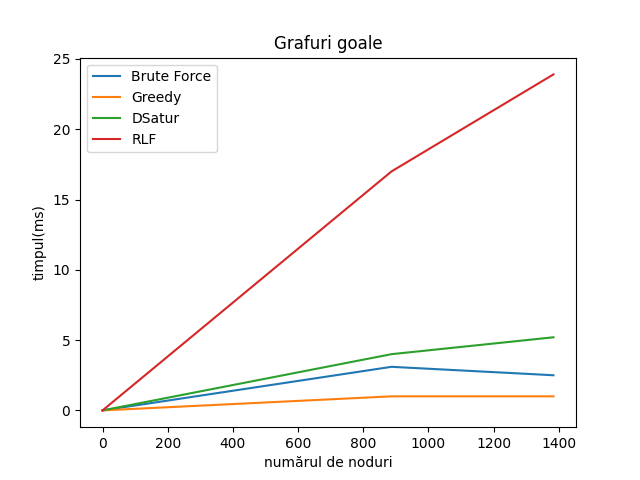
\includegraphics[width=0.8\textwidth]{./graphics/fig1.png}
\caption{Graficele timpului de rulare pentru grafuri goale}
\label{fig:empty_graphs}
\end{figure}

\begin{figure}[!]
\centering
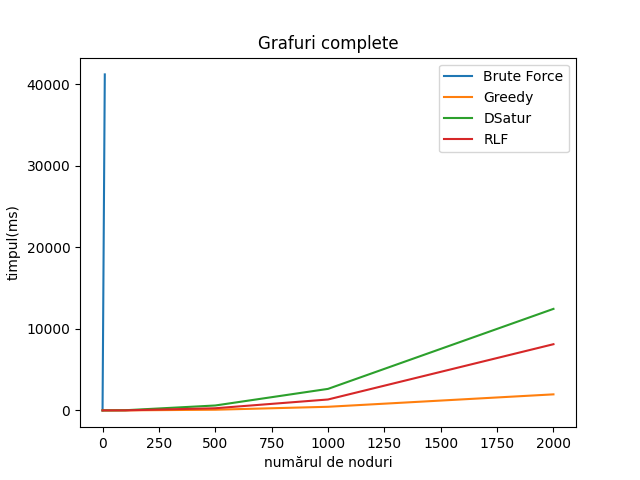
\includegraphics[width=0.8\textwidth]{./graphics/fig2.png}
\caption{Graficele timpului de rulare pentru grafuri complete}
\label{fig:complete_graphs}
\end{figure}

\begin{figure}[!]
\centering
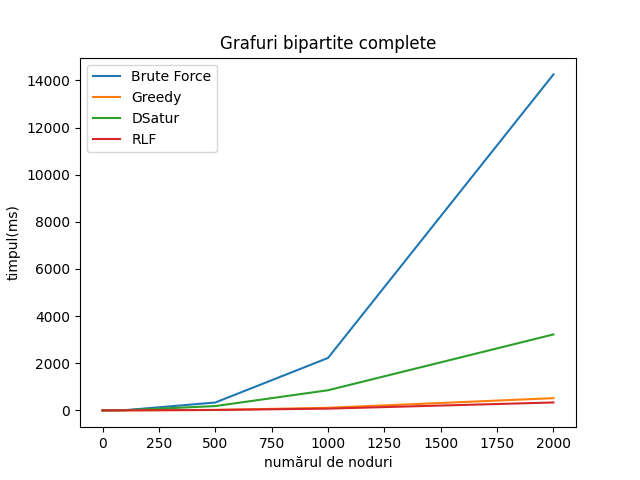
\includegraphics[width=0.8\textwidth]{./graphics/fig3.png}
\caption{Graficele timpului de rulare pentru grafuri bipartite complete}
\label{fig:bipartite_complete_graphs}
\end{figure}

\begin{figure}[!]
\centering
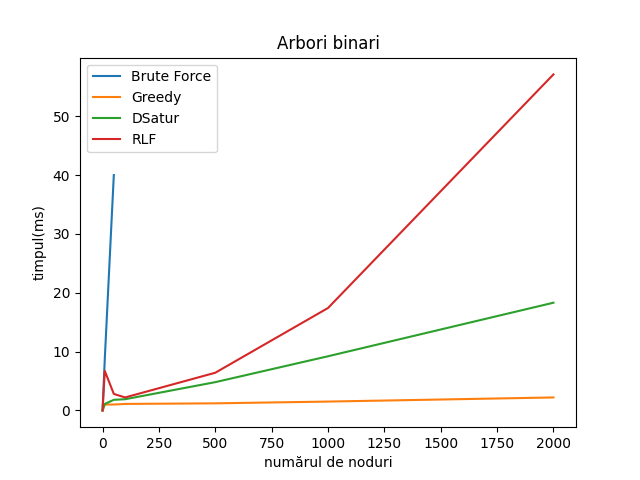
\includegraphics[width=0.8\textwidth]{./graphics/fig4.png}
\caption{Graficele timpului de rulare pentru arbori binari}
\label{fig:binary_tree_graphs}
\end{figure}

\begin{figure}[!]
\centering
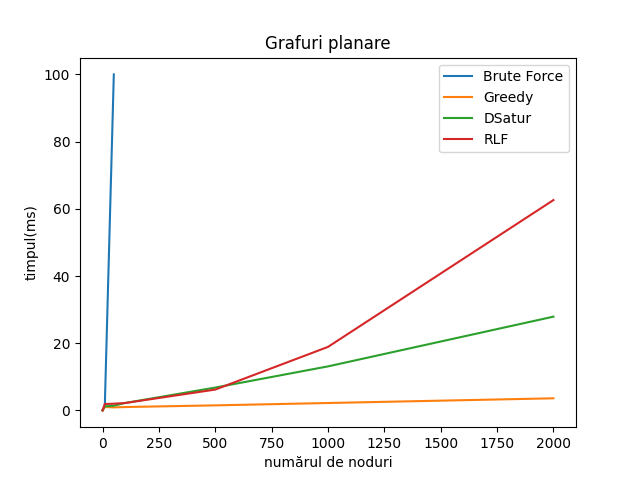
\includegraphics[width=0.8\textwidth]{./graphics/fig5.png}
\caption{Graficele timpului de rulare pentru grafuri planare}
\label{fig:planar_graphs}
\end{figure}

\begin{figure}[!]
\centering
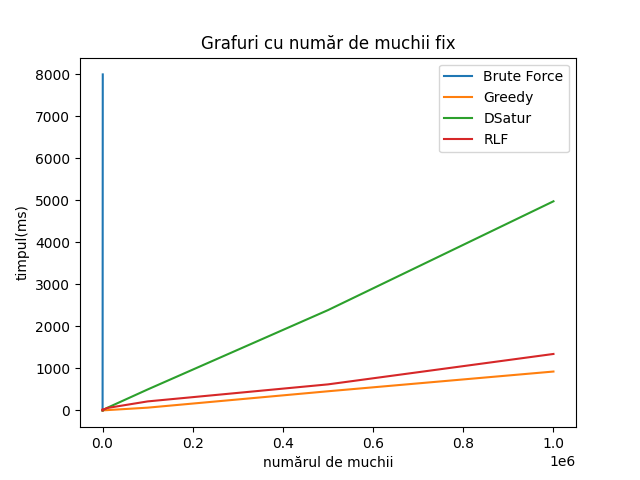
\includegraphics[width=0.8\textwidth]{./graphics/fig6.png}
\caption{Graficele timpului de rulare pentru grafuri cu număr de muchii fixat}
\label{fig:fixed_edge_number_graphs}
\end{figure}

\begin{table}[!]
\centering
\caption{Rezultatele obținute pentru fiecare set de date}
\label{tab:results}
\begin{tabular}{|c|c|c|c|c|c|c|c|}
\hline
\textbf{Nr. set} & \textbf{Nr. noduri} & \textbf{Nr. muchii} & \textbf{Nr. cromatic} & \textbf{Brute Force} & \textbf{Greedy} & \textbf{DSatur} & \textbf{RLF} \\ \hline
\textbf{1} & 887 & 0 & 1 & 1 & 1 & 1 & 1 \\ \hline 
\textbf{2} & 1384 & 0 & 1 & 1 & 1 & 1 & 1 \\ \hline
\textbf{3} & 10 & 45 & 10 & 10 & 10 & 10 & 10 \\ \hline 
\textbf{4} & 50 & 1225 & 50 & 50 & 50 & 50 & 50 \\ \hline 
\textbf{5} & 100 & 4950 & 100 & - & 100 & 100 & 100 \\ \hline 
\textbf{6} & 500 & 124750 & 500 & - & 500 & 500 & 500 \\ \hline 
\textbf{7} & 1000 & 499500 & 1000 & - & 1000 & 1000 & 1000 \\ \hline 
\textbf{8} & 2000 & 1999000 & 2000 & - & 2000 & 2000 & 2000 \\ \hline 
\textbf{9} & 10 & 21 & 2 & 2 & 2 & 2 & 2 \\ \hline 
\textbf{10} & 50 & 504 & 2 & 2 & 2 & 2 & 2 \\ \hline 
\textbf{11} & 100 & 1771 & 2 & 2 & 2 & 2 & 2 \\ \hline 
\textbf{12} & 500 & 35275 & 2 & 2 & 2 & 2 & 2 \\ \hline 
\textbf{13} & 1000 & 164151 & 2 & 2 & 2 & 2 & 2 \\ \hline 
\textbf{14} & 2000 & 557775 & 2 & 2 & 2 & 2 & 2 \\ \hline 
\textbf{15} & 10 & 9 & 2 & 2 & 3 & 2 & 3 \\ \hline 
\textbf{16} & 50 & 49 & 2 & 2 & 3 & 2 & 3 \\ \hline 
\textbf{17} & 100 & 99 & 2 & 2 & 4 & 2 & 4 \\ \hline 
\textbf{18} & 500 & 499 & 2 & - & 4 & 2 & 4 \\ \hline 
\textbf{19} & 1000 & 999 & 2 & - & 4 & 2 & 4 \\ \hline 
\textbf{20} & 2000 & 1999 & 2 & - & 4 & 2 & 4 \\ \hline 
\textbf{21} & 10 & 20 & - & 3 & 3 & 3 & 3 \\ \hline 
\textbf{22} & 50 & 100 & - & 4 & 4 & 3 & 4 \\ \hline 
\textbf{23} & 100 & 200 & - & - & 4 & 4 & 4 \\ \hline 
\textbf{24} & 500 & 1000 & - & - & 4 & 3 & 4 \\ \hline 
\textbf{25} & 1000 & 2000 & - & - & 4 & 4 & 4 \\ \hline 
\textbf{26} & 2000 & 4000 & - & - & 4 & 4 & 4 \\ \hline 
\textbf{27} & 1383 & 10 & - & 2 & 2 & 2 & 2 \\ \hline 
\textbf{28} & 886 & 100 & - & 2 & 2 & 2 & 2 \\ \hline 
\textbf{29} & 777 & 500 & - & 4 & 4 & 3 & 4 \\ \hline 
\textbf{30} & 915 & 1000 & - & - & 4 & 3 & 4 \\ \hline 
\textbf{31} & 1793 & 10000 & - & - & 8 & 6 & 8 \\ \hline 
\textbf{32} & 1386 & 100000 & - & - & 40 & 35 & 40 \\ \hline 
\textbf{33} & 1421 & 500000 & - & - & 167 & 153 & 167 \\ \hline 
\textbf{34} & 1763 & 1000000 & - & - & 276 & 258 & 276 \\ \hline 
\end{tabular}
\end{table}

\subsection{Interpretarea rezultatelor}
În raport cu timpul de execuție, avem următoarele observații:
\begin{itemize}
    \item Algoritmul Brute Force este cel mai lent, \textbf{nu} se folosește
    în practică deloc.
    \item Algoritmul Greedy pe toate tipurile de grafuri este cel mai rapid.
    \item Algoritmul DSatur este mai rapid decât algoritmul Brute Force, dar
    mai lent decât algoritmul Greedy.
    \item Algoritmul RLF pe grafuri goale este mai lent și decât algoritmul
    Brute Force, pe grafuri planare și arbori binari este mai lent decât DSatur, 
    iar pe restul de grafuri este între Greedy și DSatur (aici au apărut cazuri
    care în teorie nu sunt adevărate din cauza complexității agoritmului (vezi \ref{tabel_complexitate}).
    Acest lucru se datorează faptului că nu s-au putut genera teste suficient de
    mari și rulate de un număr suficient de ori pentru a se observa diferența dintre algoritmi.)

\end{itemize}

În raport cu numărul cromatic, se poate observa cu ușurință faptul că algoritmul
Brute Force este un algoritm exact, iar restul sunt aproximări (deși în teste 
nu se observă o diferență între numărul cromatic teoretic și rezultatul de la algoritmul DSatur, dacă
am fi avut un număr mai mare de teste cu numărul cromatic precalculat, ar fi apărut diferența).
Dintre toți1 algoritmii euristici, algoritmul DSatur este cel mai exact.

\section{Concluzii}
În cadrul acestei teme am observat 4 algoritmi diferiți de colorare a grafurilor.

Se poate afirma că nu există o soluție complet generală pentru colorarea grafurilor.
Fiecare din cele prezentate mai sus vin cu avantajele și dezavantajele lor.

Algoritmul Brute Force este cel mai lent, dar este exact, algoritmul Greedy este
cel mai rapid, dar nu este exact, algoritmul DSatur deși este mai lent decât Greedy,
este cel mai exact dintre algoritmi, iar algoritmul RLF este mai lent decât Brute Force și 
DSatur, dar este aproximativ exact.

În practică:
\begin{itemize}
    \item Dacă lucrați cu grafice bipartite sau ciclice, algoritmul Greedy nu este
    suficient de eficient; pe de altă parte, algoritmul RLF este destul de exact și total
    recomandat pentru aceste cazuri.
    \item Dacă prioritar este timpul, se poate înclina spre utilizarea algoritmul Greedy.
    \item Dacă prioritatea este un număr mai apropiat de cel cromatic, trebuie
    să se utilizeze algoritmul DSatur.

\end{itemize}
\pagebreak
% ------------------------------------------------------------------------------

%
% ---- Bibliography ----
%
% BibTeX users should specify bibliography style 'splncs04'.
% References will then be sorted and formatted in the correct style.
%
% \bibliographystyle{splncs04}
% \bibliography{mybibliography}
%
\begin{thebibliography}{8}

    \bibitem{1}
    J. Bondy and U. Murty, Graph Theory - Graduate Texts in Mathematic.
    Springer, 2008.
    \bibitem{2}
    Z. \`{A}d\`{a}m Mann and A. Szajk\`{o}, “Average-case complexity of backtrack
    search for coloring sparse random graphs,” Journal of Computer and
    System Sciences, vol. 79, no. 8, pp. 1287–1301, 2013.
    \bibitem{3}
    “Backtrack: An o(1) expected time algorithm for the graph coloring
    problem,” Information Processing Letters, vol. 18, no. 3, pp. 119–121,
    1984.
    \bibitem{4}
    N. Barnier and P. Brisset, “Graph coloring for air traffic flow management,” 
    Annals of Operations Research, vol. 130, 03 2002.
    \bibitem{5}
    “The application of a graph coloring method to an examination scheduling problem,” 
    Institute for Operations Research and the Management
    Sciences (INFORMS), vol. 11, no. 5.
    \bibitem{6}
    \href{http://www.ijimt.org/papers/359-D0129.pdf}{University Exam Scheduling System Using Graph
    Coloring Algorithm and RFID Technology}
    \bibitem{7}
    A. Murat and B. Nurdan, “A performance comparison of graph coloring algorithms,” 
    International Conference on Advanced Technology
    Sciences (ICAT’16), vol. 4, pp. 1–19, 12 2016
    \bibitem{8}
    Z. Mann, “Complexity of coloring random graphs: An experimental
    study of the hardest region,” Journal of Experimental Algorithmics,
    vol. 23, pp. 1–19, 03 2018
    \bibitem{9}
    \href{https://acs-aa-challenge.github.io/acs-aa-challenge/18-np-2-colouring/}{Enunțul problemei}
    \bibitem{10}
    M. Garey and D. Johnson, Computer and Intractability: A Guide to the
    Theory of NP-Completeness, 01 1979.
    \bibitem{11}
    D. Porumbel, J.-K. Hao, and P. Kuntz, “An evolutionary approach with
    diversity guarantee and well-informed grouping recombination for graph
    coloring,” Computers Operations Research, vol. 37, pp. 1822–1832, 10
    2010.
    \bibitem{12}
    L. Ouerfelli and H. Bouziri, “Greedy algorithms for dynamic graph coloring,” 2011 International Conference on Communications, Computing
    and Control Applications, CCCA 2011, 03 2011.
    \bibitem{13}
    \`{A}. E. Eiben, J. K. Van Der Hauw, and J. I. van Hemert, “Graph coloring
    with adaptive evolutionary algorithms,” Journal of Heuristics, vol. 4,
    no. 1, pp. 25–46, 1998.
    \bibitem{14}
    D. Br\`{e}laz, “New methods to color the vertices of a graph,”  Commun.
    ACM, vol. 22, pp. 251–256, 04 1979.
    \bibitem{15}
    R. Janczewski, K. Manuszewski, and K. Piwakowski, “The smallest
    hard-to-color graph for algorithm dsatur,” Discrete Mathematics, vol.
    236, pp. 151–165, 06 2001.
    \bibitem{16}
    \href{https://github.com/ifsmirnov/jngen}{GitHub - Jngen: preparing tests made simpler}
    \bibitem{}
    \href{https://en.wikipedia.org/wiki/Graph_coloring}{Graph coloring - Wikipedia}
    \bibitem{}
    \href{https://citeseerx.ist.psu.edu/document?repid=rep1&type=pdf&doi=203a7b17267a28a06808bfb3b0b9571e32d15503}{A Comparison of Parallel Graph Coloring Algorithms}
    \bibitem{}
    \href{https://dergipark.org.tr/en/download/article-file/254140}{A Performance Comparison of Graph Coloring Algorithms}
    % \bibitem{}
    % \href{https://github.com/brrcrites/graph-coloring}{Graph coloring C++ library}
    \bibitem{}
    \href{https://curs.upb.ro/2022/mod/folder/view.php?id=77105}{Moodle - Analiza algoritmilor}
    % 
    \end{thebibliography}
\end{document}
